\section{Schnyder Woods}\label{sw}
Schnyder Wälder, im weiteren \textit{Schnyder Woods}, wurden zuerst von Walter Schnyder zur Betrachtung der Ordnungs-Dimension planarer Graphen, als eine Färbung und Orientierung auf den inneren Kanten einer Triangulierung, betrachtet \cite{schnyder89}. In einem weiteren Resultat dienten sie zur Erlangung einer planaren Einbettung auf einem $(n-2)\times(n-2)$ Gitter \cite{schnyder90}. Dieser Abschnitt führt die Verallgemeinerung auf 3-zusammenhängende plane Graphen durch Felsner \cite{felsner01} und die zu ihnen in Bijektion stehenden Schnyder Labelings ein und orientiert sich an \cite{felsner04}.\

Für den Rest dieses Kapitels sei $G$, wenn nicht weiter spezifiziert, ein 3-zusammenhängenden planer Graph mit Aufhängungen $\{a_1,a_2,a_3\}$.

\begin{definition}[Schnyder Woods]\label{def_sw}
Ein Schnyder Wood ist eine Orientierung und Beschriftung der Kanten von $G$ mit den Labeln 1, 2 und 3\footnote{Alternativ wird hier auch anschaulicher von rot, grün und blau als Platzhalter für 1, 2 und 3 gesprochen. Es wird davon ausgegangen, dass die Label zyklisch sortiert sind, sodass $i+1$ und $i-1$ immer definiert sind.}, unter Berücksichtigung der folgenden Regeln:
\begin{itemize}
\item[W1] Jede Kante ist entweder un- oder bigerichtet. Falls sie bigerichtet ist haben beide Richtungen unterschiedliche Label.
\item[W2] An jeder Aufhängung  $a_i$ existiert eine nach aussen gerichtete Kante ohne Endpunkt mit Label i.  
\item[W3] Jeder Knoten $v$ hat hat Ausgangsgrad eins zu jedem Label. Um $v$ existieren im Uhrzeigersinn eine Auskante mit Label 1, null oder mehr eingehende Kanten mit Label 3, eine Auskante mit Label 2, null oder mehr  eingehende Kanten mit Label 1, eine Auskante mit Label 2 und null oder mehr  eingehende Kanten mit Label 2.
\item[W4] Es existiert kein inneres Gebiet mit gerichteten Zykel in einer Farbe als Rand.
\end{itemize}
\end{definition}

\begin{figure}[h]
	\centering
  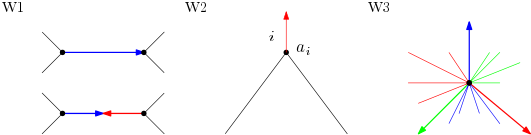
\includegraphics[width=0.8\textwidth]{schnyder_wood_def.png}
\end{figure}

Analog zu den Schnyder Woods, kann man Schnyder Labelings definieren, die zu diesen in Bijektion stehen.

\begin{definition}[Schnyder Labeling]\label{def_sl}
Ein Schnyder Labeling ist eine Beschriftung der Winkel von $G$ mit den Labeln 1, 2 und 3 unter Berücksichtigung der folgenden Regeln:
\begin{itemize}
\item[L1] Um jedes innere Gebiet bilden die Label im Uhrzeigersinn nichtleere Intervalle von 1en, 2en und 3en. Am äusseren Gebiet gilt dies gegen den Uhrzeigersinn.
\item[L2] Um jeden inneren Knoten bilden die Label im Uhrzeigersinn nichtleere Intervalle von 1en, 2en und 3en.
\item[L3] An Aufhängung $a_i$ haben äusseren Winkel die Label i-1 und i+1 im Uhrzeigersinn mit der halben Auskante dazwischen und die inneren Winkel das Label i.
\end{itemize} 
\begin{figure}[h]
	\centering
  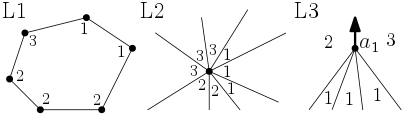
\includegraphics[width=0.8\textwidth]{schnyder_label_def.png}
\end{figure}
\end{definition}

In Abbildung \ref{schnyder_bij} wird eine Verbindung zwischen Schnyder Woods und Schnyder Labelings illustriert. Das nächste Lemma folgt aus L1 und L2.

\begin{lemma}\label{lem_sl}
Sei G ein planer, intern-3-zusammenhängender Graph mit den Aufhängungen und einem Schnyder Labeling. Dann beinhalten die vier Winkel an einer Kante die Label 1, 2 und 3. Somit hat jede Kante einen der beiden Typen in Abbildung \ref{schnyder_bij}.
\end{lemma}

\begin{figure}[h]
	\centering
  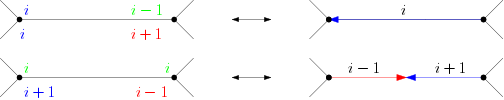
\includegraphics[width=0.7\textwidth]{schnyder_bij.png}
	\caption{Bijektion zwischen Schnyder Wood auf der rechten und Schnyder Labeling auf der linken Seite.}
	\label{schnyder_bij}
\end{figure}

Wenn wir uns auf intern-3-zusammenhängende planare Graphen beschränken, dann ist die dargestellte Abbildung nach \cite[Theorem 2.3]{felsner04} eine Bijektion. \\

Es existieren einige Anwendungen von Schnyder Woods im Bezug auf Einbettungen. Eine ist das im Folgenden skizzierte \textit{face-counting} \cite{felsner01}. Betrachte $G$ mit einem Schnyder Wood $T_1,T_2,T_3$. Nach \cite[Korollar 2.5]{felsner04} handelt es sich bei den $T_i$ um gerichtete Bäume mit Wurzeln in $a_i$. Von jedem Knoten $v$ aus existierten also eindeutige Pfade $P_i(v)$ zu den Aufhängungen $a_i$. Die Pfade von $v$ zu den Aufhängungen treffen sich nach \cite[Lemma 2.4]{felsner04} nur in $v$. Somit können wir zu jedem Knoten $v$ die von den Pfaden $P_{i-i}(v)$ und $P_{i+1}(v)$ und dem äusseren Gebiet begrenzte Region $R_i$ betrachten. Durch das Zählen der Gebiete in den Regionen zu $v$ lässt sich nun eine konvexe Zeichnung von $G$ erzeugen. \

Hierzu ordnet man jedem Knoten $v$ seien Gebiets Vektor $(v_1,v_2,v_3)$ zu, wobei $v_i$ die Anzahl der inneren Gebiete in $R_i(v)$ beschreibt. Nun gilt für jeden Knoten $v_1+v_2+v_3 = |F|-1$. Seien $\alpha_1 = (0,1),\alpha_2 = (1,0)$ und $\alpha_3 = (0,0)$ die äusseren Ecken unserer Zeichnung, dann erhalten wir die Position der inneren Knoten durch die Funktion 
$$\mu:v\to v_1\alpha_1 + v_2\alpha_2+v_3\alpha_3.$$ 

Nach \cite[Theorem 2.7]{felsner04} ist die mit diesen Koordinaten erzeugte Zeichnung planar und konvex und passt auf ein $(|F|-1)\times(|F|-1)$-Gitter. Sie hat noch eine weitere Eigenschaft die später von Nutzen ist.

\begin{itemize}
\item [W5] Die Knoten eines inneren Gebietes werden auf die Seiten eines Dreiecks mit den Seiten $c_i(\alpha_{i-1}-\alpha_{i+1})$ mit passenden Konstanten $c_i$. Im inneren dieses Dreiecks befinden sich keine Knoten und die Winkel des Gebietes auf der Seite $c_i(\alpha_{i-1}-\alpha_{i+1})$ haben Label $i$ im Schnyder Labeling.
\end{itemize}

\begin{figure}[h]
	\centering
  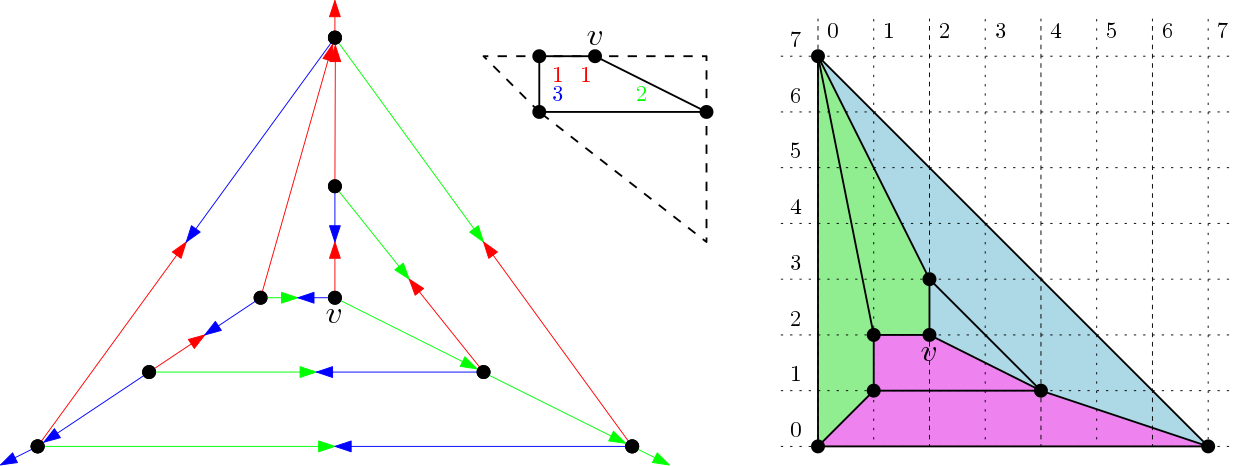
\includegraphics[width=0.8\textwidth]{face_counting.png}
	\caption{Eine Schnyder Wood und die durch \textit{face counting} erhaltene Einbettung. Die eingefärbten Gebiete sind die Regionen die den Gebietsvektor $(v_1,v_2,v_3)$ ergeben. In der Mitte ist W5 illustriert.}
	\label{face_counting}
\end{figure}
